\documentclass[12pt,tikz]{standalone}
\pdfinfoomitdate 1
\pdfsuppressptexinfo 1
\pdftrailerid{}
\usepackage[utf8]{inputenc}
\usepackage{amsmath}
\usepackage{pgfplots}
\usepackage{tikz}
\usetikzlibrary{shapes.geometric}
\pagestyle{empty}

\begin{document}
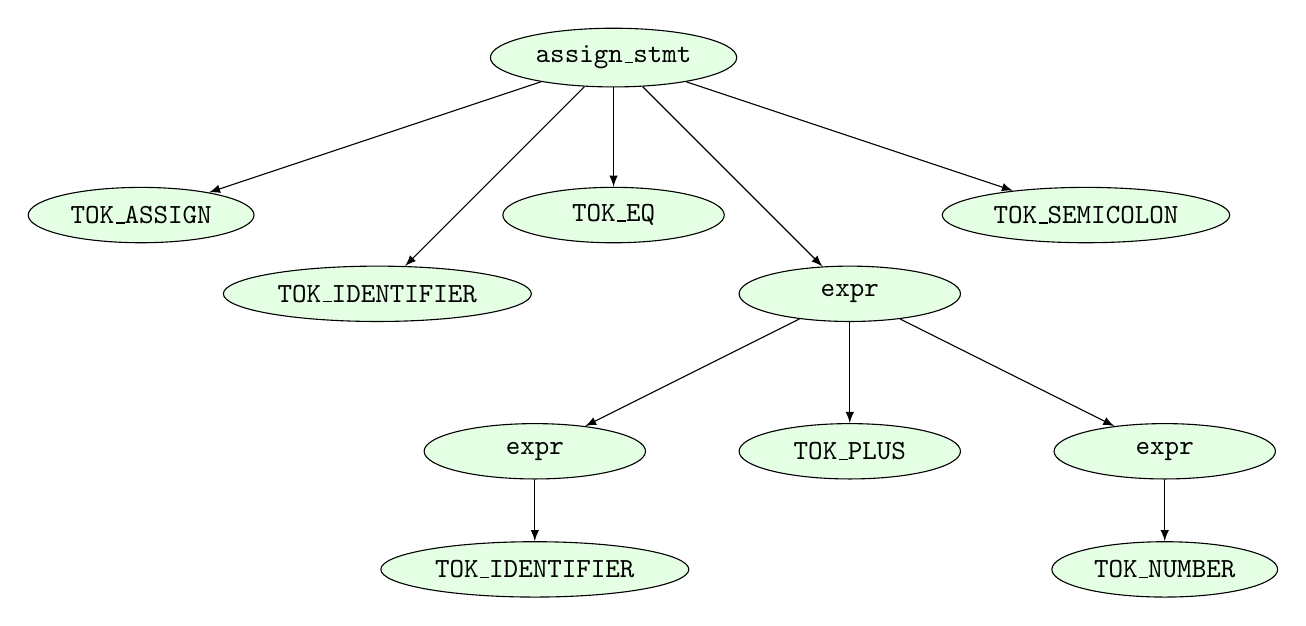
\begin{tikzpicture}
	\tikzstyle{node} = [draw, fill=green!10, ellipse, minimum height=2em, minimum width=8em, node distance=10em]

	\draw (+0,+1) node[node] (n1) {\tt assign\_stmt};

	\draw (-6,-1) node[node] (n11) {\tt TOK\_ASSIGN};
	\draw (-3,-2) node[node] (n12) {\tt TOK\_IDENTIFIER};
	\draw (+0,-1) node[node] (n13) {\tt TOK\_EQ};
	\draw (+3,-2) node[node] (n14) {\tt expr};
	\draw (+6,-1) node[node] (n15) {\tt TOK\_SEMICOLON};

	\draw (-1,-4) node[node] (n141) {\tt expr};
	\draw (+3,-4) node[node] (n142) {\tt TOK\_PLUS};
	\draw (+7,-4) node[node] (n143) {\tt expr};

	\draw (-1,-5.5) node[node] (n1411) {\tt TOK\_IDENTIFIER};
	\draw (+7,-5.5) node[node] (n1431) {\tt TOK\_NUMBER};

	\draw[-latex] (n1) -- (n11);
	\draw[-latex] (n1) -- (n12);
	\draw[-latex] (n1) -- (n13);
	\draw[-latex] (n1) -- (n14);
	\draw[-latex] (n1) -- (n15);

	\draw[-latex] (n14) -- (n141);
	\draw[-latex] (n14) -- (n142);
	\draw[-latex] (n14) -- (n143);

	\draw[-latex] (n141) -- (n1411);
	\draw[-latex] (n143) -- (n1431);
\end{tikzpicture}
\end{document}
